\documentclass[../PS6_RapportFinal.tex]{subfiles}

\begin{document}
\graphicspath{{img/}{tex/img/}}
\subsection{Résultats}

Nous avons utilisé les valeurs trouvées expérimentalement pour la concentration initiale de réactif, la conductivité thermique et la capacité thermique (partie \ref{mesurecaracteristiques}). Par identification inverse, nous cherchons les valeurs de l'énergie d'activation et de la constante de réaction $k_{reac}$ du modèle.

Nous avons commencé par tester le simulateur avec une simple diffusion de chaleur sans terme source, et les résultats étaient corrects. Nous sommes donc passés à la réelle phase de simulation.
Au début, les résultats semblaient aberrants : la réaction semblait durer très longtemps (voir figure \ref{concentration_trop_grande}), quelques soient les valeurs de $E_{a}$ et $k_{reac}$, ce qui ne correspondait pas à la réalité de ce que nous voyions. Nous avons résolu le paradoxe en choisissant de mettre uniquement un centième de la valeur théorique de la concentration en réactif. Le résultat a été beaucoup plus cohérent avec nos observations (voir figure \ref{concentration_un_centieme}), ce qui nous permet de déduire que seul environ 1\% du bois composte réellement et produit de la chaleur. Étant donné l'état dans lequel nous trouvons le compost à la fin de l'expérience (trop sec ou peu dégradé dans la plupart des zones de la cuves), cette estimation semble plausible.

\begin{figure}[!h]
\begin{center}
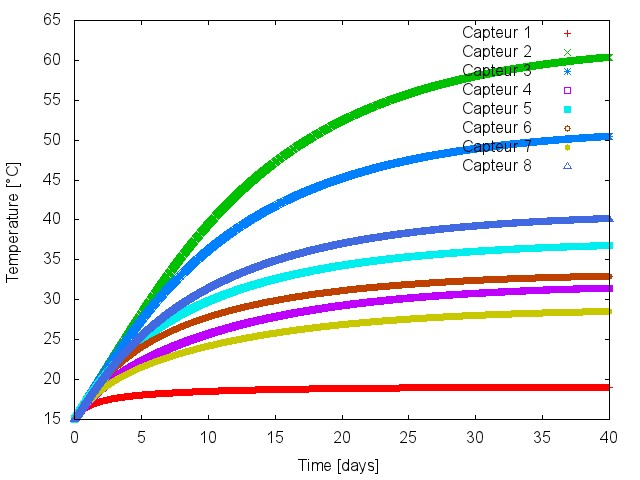
\includegraphics[height=8cm]{2_4_concentration_trop_grande.jpg}
\caption{Profil de température simulé pour $C_{ini} = C_{th}$}
\label{concentration_trop_grande}
\end{center}
\end{figure}

\begin{figure}[!h]
\begin{center}
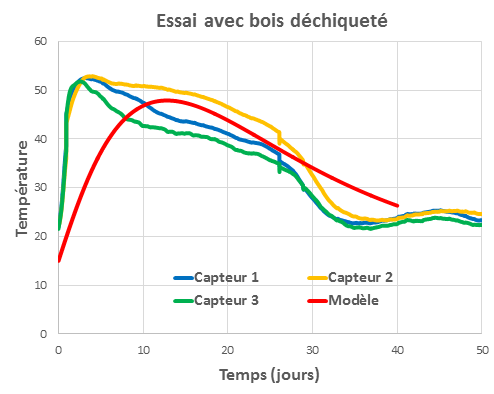
\includegraphics[width=10cm]{2_4_Essai_septembre.png}
\caption{Profil de température réel pour une cuve de bois déchiqueté et simulé pour $C_{ini} = \frac{C_{th}}{100}$}
\label{concentration_un_centieme}
\end{center}
\end{figure}


\end{document}